\documentclass{beamer}

%\usetheme{Darmstadt}
\usepackage{beamerthemesplit}
\usepackage{graphicx}
\usepackage{amsmath,amsfonts,dsfont}
\def\ev {\mbox{E}}
\def\mse {\mbox{MSE}}
\def\var {\mbox{Var}}
\def\bias {\mbox{Bias}}

\pgfdeclareimage[height=10mm]{logo}{EURACE-Flag.png}

\title{Agent-based economic modelling in EURACE}
\titlegraphic{\pgfuseimage{logo}}
\author{Marco Raberto}
%\logo{\pgfuseimage{logo}}

\vspace{0.3cm}
\institute{Reykjavik University, Iceland\\and\\The EURACE Consortium, University of Genoa, Italy}


\date{}

\begin{document}

\section{EURACE Winter School, Genoa, 18-21 November 2009}
%\part{EURACE Winter School, Genoa, 18-21 November 2009}

\frame{\titlepage}

\section{}

\frame{
  \frametitle{Summary}
  \begin{itemize}
     \item Introduction to the ACE approach
      \vspace{0.2cm}
   \item Key features of EURACE
      \vspace{0.2cm}
   \item Agents
      \vspace{0.2cm}
   \item Timing
      \vspace{0.2cm}
      \item Markets
      \vspace{0.2cm}
   \item The balance sheet approach
         \vspace{0.2cm}
    \item Concluding remarks
  \end{itemize}

}

\frame{
  \frametitle{A snapshot of EURACE}
  \begin{itemize}
   \item The EURACE model is by far the largest and most complete agent-based model developed in the world to date.
        \vspace{0.3cm}
   \item It represents a fully integrated macroeconomy consisting of:
\begin{itemize}
  \vspace{0.2cm}
   \item the \textbf{real sector} (production of consumption and capital goods with labor, capital goods and energy as factors of production and relative markets; technological innovation);
     \vspace{0.2cm}
   \item the \textbf{credit sector} (financing production plans of firms);
     \vspace{0.2cm}
        \item the \textbf{financial sector} (exchange of claims on the equity capital of producers as well as of governments liabilities);
     \vspace{0.2cm}
   \item the \textbf{public sector} (polcy making, i.e., fiscal policy made by Governments and monetary policy set by the Central Bank).
  \end{itemize}
  \end{itemize}
}

\frame{
  \frametitle{Main objectives of EURACE}
  \begin{itemize}
   \item Scientific objectives:
   \begin{itemize}
   \item Establishing an innovative framework for the study of the macroeconomy according to the agent-based computational approach.
   \vspace{0.2cm}
    \item Providing new insights on the emergence of global regularities in the aggregation of heterogeneous interacting agents.
   \end{itemize}
   \vspace{0.2cm}

   \item Technological objective:
   \begin{itemize}
   \item Development of new software methodologies for implementing, designing and validating large-scale agent-based economic simulations.
   \end{itemize}

   \vspace{0.2cm}
   \item Societal objective:
   \begin{itemize}
    \item Development of an agent-based software platform to perform simulation experiments on economic policy design for the European Union.
   \end{itemize}

  \end{itemize}
}


\frame{
  \frametitle{Why EURACE ?}
  \begin{itemize}
   \item In 2005, when the proposal was presented to EU, we were unsatisfied about the present state of mainstream economic theory (representative agents,  rational expectations, perfect asset markets, market clearing, ...)

   \vspace{0.5cm}

   \item 2009: what about now?

  \end{itemize}
}

\frame{
  \frametitle{2009: the  state of the mainstream approach :-)}
\begin{figure}
  % Requires \usepackage{graphicx}
 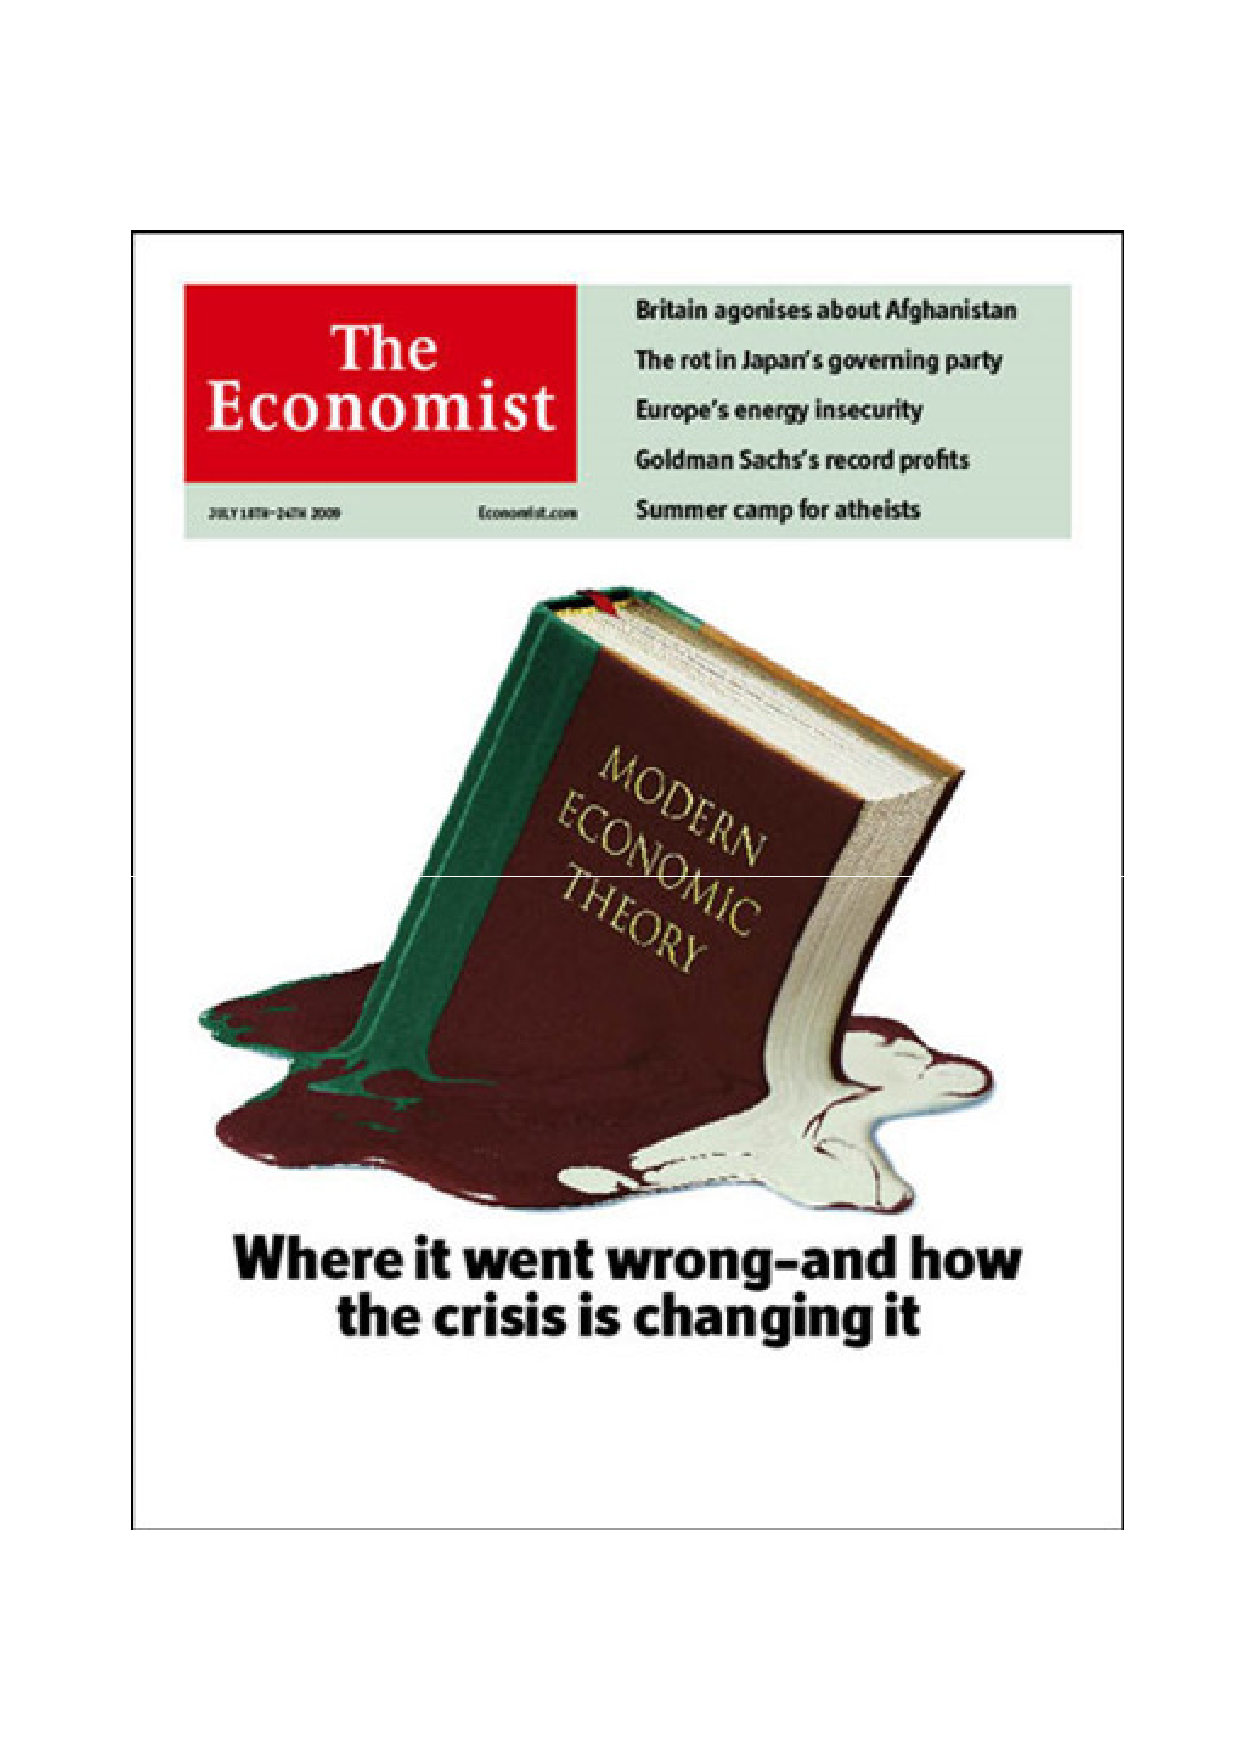
\includegraphics[width=0.5\textwidth]{economist_cover.pdf}\\
\end{figure}

}

\frame{
  \frametitle{The day after the crisis.....}
\begin{itemize}
  \item The current financial and banking crisis and the subsequent severe economic recessions have caused a crisis of confidence in the science of Economics.
     \vspace{0.3cm}

  \item Most economists have been unable to forecast timely the crisis and even to devise helpful policies at its beginning.
         \vspace{0.3cm}

  \item The Nobel Laureate Paul Krugman recently feared that most macroeconomics of the past 30 years was ``spectacularly useless at best, and positively harmful at worst" (The Economist, July $16^{th}$ 2009).
   \vspace{0.2cm}

   \item ``Economics needs a scientific revolution" by J.-P. Bouchaud (Nature, October $30^{th}$, 2008)

   \end{itemize}
}


\frame{
  \frametitle{Why mainstream failed to predict the crisis?}

 \begin{itemize}

  \item According to mainstream approaches to economics, e.g. DSGE models, the structure of financial liabilities in the economy only has limited influence on the aggregate economic activity.
     \vspace{0.2cm}

      \item Capitalist economies are viewed as essentially stable and tending towards steady growth; and the investment-finance linkage is considered at the most as amplifying mechanism of exogenous shocks.
     \vspace{0.2cm}

  \item On the contrary, a different, unduly neglected strand of research emphasizes the role of the investment-finance link not just as a propagator of exogenous shocks but as the main source of financial instability and business cycles. (H. Minsky, Stabilizing an Unstable Economy, 1986).

     \vspace{0.2cm}

 \end{itemize}

}

\frame{
  \frametitle{The ACE approach}

 \begin{itemize}

\item Simulating artificial economies on the computer is becoming a promising approach to the study of economic systems, able to overcome the limitations of elegant, yet unrealistic, mainstream analytical economic models (Nature vol 460, August 2009).
\vspace{0.2cm}

\item The study of the economy by means of agent-based computational models is a relatively new field and dates back to the 90s.

\vspace{0.2cm}
     
\item The increasing availability of cheap computing power made possible to undertake the computationally expensive experiments required to model the interactions of large numbers of bounded rational, heterogeneous agents.

 \end{itemize}

}


\frame{
  \frametitle{The ACE approach and the credit crisis}

 \begin{itemize}

\item The agent-based methodology fully addresses the interaction and the coordination processes of heterogeneous economic agents by considering both individual and social learning behaviours.
\vspace{0.2cm}

\item It allows the study of the emergent aggregate statistical regularities in the economy, which cannot be originated by the behaviour of a ``typical" or ``average" individual (Kirman J. Econ Perspectives 1992), but is the result of agents' behaviour and interaction.

\vspace{0.2cm}

\item It takes into account the complex pattern of interactions in the credit markets, like networks topologies, credit rationing, bankruptcy waves and cascade effects, which are very important issues for the present state of the economy.

 \end{itemize}

}


\frame{
  \frametitle{Example: financial fragility under the ACE approach}

 \begin{itemize}

\item Relevant examples today are the studies about the relationship between financial fragility of firms and business fluctuations (Delli Gatti et al. JEBO 2005). 

\vspace{0.2cm}
    
\item If firms are heterogeneous (also) in terms of degree of financial fragility, this type of heterogeneity plays a crucial role in the evolution over time of aggregate variables such as production and unemployment. 

\vspace{0.2cm}
    
\item In this context, small idiosyncratic shocks at firm-level may generate single firm bankruptcies, which cause credit rationing by banks and so waves of bankruptcies among firms, then inducing large aggregate fluctuations in the economy.

\vspace{0.2cm}

\item Furthermore, an endogenous credit bubble and then a boom-bust cycle caused by overlending during good times may be created and studied.

 \end{itemize}

}

\frame{
  \frametitle{The ACE approach for policy design}

\begin{itemize}


\item Multi-agent economic systems are gaining more and more attention for the purpose of policy analysis. 

\vspace{0.1cm}
    
\item An agent-based simulator is a powerful computational facility where to perform large-scale experiments on complex and realistic economic environments and to test different issues of policy design.

\vspace{0.1cm}

\item It offers a realistic environment that is well suited for studying the out-of-equilibrium transitory dynamics of the economy caused by changes of policy parameters.

\vspace{0.1cm}

\end{itemize}    
See e.g., two special issues: Dawid and Fagiolo, eds, 2008 and LeBaron and Winker, eds, 2008). Some studies are focused on the design of regulatory policies for financial markets (Mannaro et al. 2008, Westerhoof et al. 2008), other on the design of appropriate fiscal and monetary policies. (Russo et al. 2007; Haber 2008, Raberto et al. 2006, Raberto et al. 2008)



}

\frame{
  \frametitle{Key features of EURACE}
  \begin{itemize}
      \item Technology (FLAME, GUIs, parallelization).
   \vspace{0.2cm}
      \item Spatial structure and local interactions.
   \vspace{0.2cm}
     \item Realistic time scales and asynchronous interactions.
   \vspace{0.2cm}
   \item Decentralized markets (Walasian auctioneer banned expect for the financial market):
       \begin{itemize}
      \item market clearing is not for granted
  \item no law of one price
\end{itemize}
 \vspace{0.2cm}
   \item Adaptive and empirically grounded behavioral rules (optimization banned).
   \vspace{0.2cm}
    \item Balance sheet approach in modeling agents.
   \vspace{0.2cm}
   \item Validation based on the reproducibility of well-known empirical regularities and the consistency of balance sheets.
  \end{itemize}
}


\frame{
  \frametitle{Agents (I)}
  The EURACE model is characterized by a set of agents' typologies with proper balance sheets and behavioral features:
  \vspace{0.2cm}
  \begin{itemize}
   \item Households
   \vspace{0.2cm}
   \item Consumption goods producing firms
   \vspace{0.2cm}
   \item Investment goods producing firms
   \vspace{0.2cm}
   \item Commercial Banks
   \vspace{0.2cm}
   \item Governments
   \vspace{0.2cm}
   \item Central bank
  \end{itemize}
}


\frame{
  \frametitle{Agents (II)}
  Besides the agents presented before, the simulator is populated by a number of agents for the  purpose of facilitating market exchanges and statistical computation:
    \vspace{0.4cm}
  \begin{itemize}
   \item Malls
     \vspace{0.2cm}
   \item Eurostat
     \vspace{0.2cm}
   \item Clearing House
  \end{itemize}
}


\frame{
  \frametitle{Households}
They have the role of:
     \vspace{0.2cm}
  \begin{itemize}
   \item consumers
     \vspace{0.2cm}
   \item workers
     \vspace{0.2cm}
     \item firms' equity and governments' debt holders
     \vspace{0.2cm}
     \item financial traders
  \end{itemize}
}

\frame{
  \frametitle{Firms}
  \begin{itemize}
   \item Consumption Goods Producers
     \vspace{0.1cm}
    \begin{itemize}
       \item Employ labor and capital goods to produce consumption goods
         \item They sell consumption goods to households
       \vspace{0.1cm}
       \item Take loans from commercial banks to finance their production plans
       \vspace{0.1cm}
       \item Distribute dividends to shareholders (households)
     \end{itemize}

     \vspace{0.3cm}

   \item Investment Goods Producers
    \begin{itemize}
       \item Employ labor and energy to produce capital goods
       \vspace{0.1cm}
       \item They sell capital goods to consumption goods producers
       \vspace{0.1cm}
       \item Distribute dividends to shareholders (households)
     \end{itemize}
   \end{itemize}
}


\frame{
  \frametitle{Commercial banks}
     \vspace{0.2cm}
  \begin{itemize}
   \item Collect cash deposits from households and firms
     \vspace{0.2cm}
   \item Give loans to firms
     \vspace{0.2cm}
     \item Access the standing facility of the the central bank
     \vspace{0.2cm}
     \item Distribute dividends to shareholders (households)
  \end{itemize}
}


\frame{
  \frametitle{Policy makers: Governments and the Central Bank}
     \vspace{0.2cm}

\begin{itemize}
\item Governments:
  \vspace{0.2cm}
  \begin{itemize}
\item Decide fiscal policies (set tax rates)
  \vspace{0.2cm}
\item Collect taxes
  \vspace{0.2cm}
\item Pay unemployment benefits, transfer and subsidies
  \vspace{0.2cm}
\item Issue bonds to finance budget deficit
  \end{itemize}

  \vspace{0.4cm}

\item Central Bank:
  \vspace{0.2cm}
  \begin{itemize}
\item Decide monetary policies (set interest rates and eventually implement quantitative easing by means of government bonds purchase)
  \vspace{0.2cm}
\item Provide temporary liquidity if needed to Governments and Commercial Banks (standing facility)
  \vspace{0.2cm}
  \end{itemize}
\end{itemize}

}


\frame{
  \frametitle{Timing}
\begin{itemize}
  \item The choice of time scales for the agents� decision making has been made in order to reflect the real time scales in economic activities
        \vspace{0.2cm}
  \item The agents� financial decisions are made on a shorter time
scale (day) than the economic decision making, e.g., consumption and production, where the
proper time horizon can be a week, a month, or a quarter.
\vspace{0.2cm}

\item Central bank sets its monetary policy on a monthly basis.
\vspace{0.2cm}
\item Governments decide fiscal policy on a yearly basis.

\end{itemize}
}


\frame{
  \frametitle{Asynchronous interactions}
\begin{itemize}
  \item In reality, most human decision-making and interaction is asynchronous, due to the autonomous decisions of the agents.
      \vspace{0.2cm}
  \item We model this asynchronous decision making by letting agents have different activation days.
      \vspace{0.2cm}
  \item This means that on a single market different agents are active on different days
  \vspace{0.2cm}
  \item Some activities, however, are synchronized. This is in particular the case when they are institutionally initiated (e.g., tax and wage payments).
\end{itemize}
}


\frame{
  \frametitle{Markets}
  \begin{itemize}
   \item Consumption goods market
     \vspace{0.2cm}
   \item Investment goods market
     \vspace{0.2cm}
   \item Credit market
     \vspace{0.2cm}
   \item Financial market (stock and government bonds)
     \vspace{0.2cm}
   \item Labor market
  \end{itemize}
    \vspace{0.3cm}
Except for the financial market, the other markets are all decentralized.
}


\frame{
  \frametitle{Consumption goods market}
  \begin{itemize}
   \item Consumption goods producers offer (and store) goods at selected geographically distributed local market outlets (malls).
     \vspace{0.3cm}
   \item Consumers visit their local mall and make purchasing decisions based on price/quality information they collect about the goods offered at the mall.
     \vspace{0.3cm}
   \item Suppliers on the consumption goods market act globally (without spatial frictions) whereas consumers buy locally.
     \vspace{0.3cm}
     \item Timing: asynchronous
  \end{itemize}
}


\frame{
  \frametitle{Credit market}
  \begin{itemize}
   \item Firms ask for credit to banks to finance their production plan.
     \vspace{0.2cm}
   \item Banks offer loans to firms with a related interest rate. Based on firms financial fragility, credit rationing may occur.
     \vspace{0.2cm}
   \item Firms accept loan offers according to the interest rate.
     \vspace{0.2cm}
    \item Timing: asynchronous.
  \end{itemize}
}


\frame{
  \frametitle{Financial market}
  \begin{itemize}
   \item Households form beliefs about expected assets total returns.
     \vspace{0.2cm}
   \item Households compute a desired portfolio allocation according to their preference structure.
     \vspace{0.2cm}
   \item Firms may issue new stocks to finance their production plans.
     \vspace{0.2cm}
   \item Governments may issue new bonds to finance the budget deficit.
     \vspace{0.2cm}
   \item A centralized mechanism (clearing house) collect all orders, match demands and supply curves for each assets, and clear the market.
     \vspace{0.2cm}
     \item Timing: day
  \end{itemize}
}


\frame{
  \frametitle{Labor market}
  \begin{itemize}
   \item Firms post job vacancies based on planned output.
     \vspace{0.2cm}
   \item Searching workers send applications based on posted salaries.
     \vspace{0.2cm}
   \item Firms rank applications based on skills and make offers.
     \vspace{0.2cm}
   \item Workers rank offers (wage - commuting costs), compare best offer to their reservation wage and accept/reject.
     \vspace{0.2cm}
   \item Labor Market is global with spatial frictions.
    \vspace{0.2cm}
    \item Timing: asynchronous.
  \end{itemize}
}

\frame{
  \frametitle{Examples of decision rules}
  \begin{itemize}
   \item Firms and Households act rule-based using backward looking expectations
     \vspace{0.2cm}
   \item Households decisions in the financial market are based on prospect theory
     \vspace{0.2cm}
   \item Operational decisions of firms are modelled using standard decision rules from the Operations Management literature:
       \begin{itemize}
         \item Pricing (markup)
         \item Inventory and Production Planing
       \end{itemize}
     \vspace{0.2cm}
   \item Savings/consumption decisions of household are based on empirically-founded rules derived from the buffer-stock theory of consumption, see Deaton (1991) and Carrol (1993)
     \vspace{0.2cm}
   \item    Purchasing decisions of households are modelled using standard logit-models from the Marketing literature

  \end{itemize}
    \vspace{0.3cm}
}


\frame{
  \frametitle{The balance sheet approach}
  \begin{itemize}
   \item A double-entry balance sheet with a detailed account of all monetary and real assets as well as monetary liabilities is defined for each agent.
    \vspace{0.2cm}
   \item Monetary and real flows given by agents' behaviors and interactions determine the period by period balance sheet dynamics.
    \vspace{0.2cm}
   \item A stock-flow model is then created and used to check that all monetary and real flows are accounted for, and that all changes to stock variables are consistent with these flows.
    \vspace{0.2cm}
   \item This provides us with a solid and economically well-founded methodology to test the consistency of the model and it increases the credibility that can be attached to the model's results.
  \end{itemize}
}


\frame{
  \frametitle{Monetary and financial assets}
  \begin{itemize}
     \item cash holdings in the form of commercial bank or central bank deposits. There is
no cash hoarding since all money is held inside the banking sector;
    \vspace{0.2cm}
     \item bank loans
         \vspace{0.2cm}
     \item central bank standing facility
         \vspace{0.2cm}
     \item government bonds
         \vspace{0.2cm}
     \item equity shares (issued by firms and banks)
\end{itemize}
}


\frame{
  \frametitle{Real assets}
  \begin{itemize}
     \item firms inventories
    \vspace{0.2cm}
     \item physical capital
         \vspace{0.2cm}
     \item human capital

\end{itemize}
}


\frame{
  \frametitle{Household (H): balance sheet overview}
\begin{table}
  \centering
  \begin{tabular}{|l|l|}
  \hline
  % after \\: \hline or \cline{col1-col2} \cline{col3-col4} ...
 \textbf{Assets}  &  \textbf{Liabilities} \\ \hline
   &\\
   $M^h$: liquidity deposited at a given \emph{bank} & \\
   &\\
   $n^h_g$:  government bonds holdings & (nome)\\
   &\\
   $n^h_f$, $n^h_b$:  equity shares holdings of  & \\
   \hspace{1.1cm} firm $f$ and bank $b$ & \\
  \hline
\end{tabular}
\end{table}
\begin{itemize}
\item Financial wealth:
$$W = M^h + \sum_{f \in \{firms\}} n^h_f p_f + \sum_{b \in \{banks\}} n^h_b p_b  + \sum_{g \in \{ governments\}} n^h_g p_g$$
 \item $p_f$, $p_b$: daily price of equity shares  issued by firm $f$ and bank $b$, respectively
 \item $p_g$: daily price of the bond issued by government $g$
\
\end{itemize}
}


\frame{
  \frametitle{Firm (f): balance sheet overview (I)}
\begin{table}
  \centering
  \begin{tabular}{|l|l|}
  \hline
  % after \\: \hline or \cline{col1-col2} \cline{col3-col4} ...
 \textbf{Assets}  &  \textbf{Liabilities} \\ \hline
     &  \\
   $M^f$: liquidity deposited at a given \emph{bank} & $D^f_b$: debts to \emph{banks} \\
    &  \\
   $I^f_m$: inventories at \emph{malls} & $E^f$: equity\\
    &  \\
   $K^f$: physical capital &  \\
  \hline
\end{tabular}
\end{table}
  \vspace{0.4cm}
\begin{itemize}
  \item $M^f$, $I^f_m$ updated daily following firms' cash flows and sales
  \vspace{0.4cm}
  \item $K^f$, and $D^f_b$ updated updated monthly (at the first day of the month to act)
\end{itemize}
}


\frame{
  \frametitle{Firm (f): balance sheet overview (II)}
\begin{itemize}
    \item $E^{f}$: equity updated monthly (at the last day of the month to act) according to:
  $$E^{f} = M^{f} + p_C \sum_{m \in \{ malls\}} I^f_m + p_K K^f -\sum_{b \in \{ banks\}} D^f_b$$
   \vspace{0.4cm}
  \item $p_C$: average price level of consumption goods
   \vspace{0.4cm}
  \item $p_K$: price of capital goods
\end{itemize}
}


\frame{
  \frametitle{Bank (b): balance sheet overview (I)}
\begin{table}
  \centering
  \begin{tabular}{|l|l|}
  \hline
  % after \\: \hline or \cline{col1-col2} \cline{col3-col4} ...
 \textbf{Assets}  &  \textbf{Liabilities} \\ \hline
    & \\
   $M^b$: liquidity (reserves) & $D^{b}$: standing facility \\
   \hspace{0.7cm} deposited at the \emph{central bank} & \hspace{0.7cm}  (debts to the \emph{central bank}) \\
     & \\
   $L^b_f$: loans to firms & $M^b_h$: households' deposits \\
    & \hspace{0.6cm} at the bank \\
      & \\
    & $M^b_f$: firms' deposits at the bank \\
      & \\
   & $E^b$: equity\\
  \hline
\end{tabular}
\end{table}
}


\frame{
  \frametitle{Bank (b): balance sheet overview (II)}

\begin{itemize}

\item $M^b_h$, $M^b_f$, $L^b_f$ updated daily following the private sector deposits changes and the credit market outcomes

\vspace{0.3cm}

\item $M^b$, $E^b$ updated daily following banks cash flows and also:

$$M^b = D^b + \sum_{h \in \{ households\}} M^b_h + \sum_{f \in \{ firms\}} M^b_f + E^b - \sum_{f \in \{ firms\}} L^b_f$$

\vspace{0.3cm}

\item if $M^b$ becomes negative $D^b$ is increased to set $M^b = 0$

\vspace{0.3cm}

\item if both $M^b$ and $D^b$ are positive, $D^b$ is partially or totally repaid
\end{itemize}
}


\frame{
  \frametitle{Government (g)}
\begin{table}
  \centering
  \begin{tabular}{|l|l|}
  \hline
  % after \\: \hline or \cline{col1-col2} \cline{col3-col4} ...
 \textbf{Assets}  &  \textbf{Liabilities} \\ \hline
  & \\
   $M^g$: liquidity deposited at the   & $D^g$: standing facility with the\\
   \hspace{0.7cm} central bank & \hspace{0.7cm} central bank\\

    & $n^g$: number of outstanding bonds\\
  \hline
\end{tabular}
\end{table}
\vspace{0.3cm}
Government budget:
\begin{itemize}
\item Revenues: taxes on corporate profits and household labor and capital income;

\item Expenses: unemployment benefits, transfer and subsidies.
\end{itemize}
}



\frame{
  \frametitle{Central Bank (c): balance sheet overview (I)}
\begin{table}
  \centering
  \begin{tabular}{|l|l|}
  \hline
  % after \\: \hline or \cline{col1-col2} \cline{col3-col4} ...
 \textbf{Assets}  &  \textbf{Liabilities} \\ \hline
 & \\
   $n^{c}_g$: Government bonds (QE)  & $M^c$: fiat money due to QE\\
 & \\
   $M^{c}$: liquidity & $M_g^c$: Governments liquidity \\
    & \\
   $L^{c}_b$: loans to banks & $M_b^c$: banks reserves\\
    & \\
   $L^{c}_g$: loans to governments & $E^c$: equity\\
  \hline
\end{tabular}
\end{table}

\begin{itemize}
\item With quantitative easing (QE), the central bank purchases government bonds using money it creates from nothing (fiat money), and so expands its balance sheets.
\end{itemize}
}



\frame{
  \frametitle{Central Bank (c): balance sheet overview (II)}

\begin{itemize}
\item Since the Central Bank is not allowed to make a profit, its revenues from
government bonds and bank advances are distributed to the government in
the form of a dividend.

\vspace{0.5cm}

\item In case of multiple governments, the total dividend payment
is equally divided among the governments.
\end{itemize}
}


\frame{
  \frametitle{Validation rules}

\begin{itemize}
\item Balance sheet accounting identities can be devised across agents and used to validate the model.

\vspace{0.2cm}

\item Examples:

$$\sum_f \sum_b L^b_f = \sum_f \sum_b D^f_b $$

$$\sum_h M^h = \sum_b \sum_h M^b_h $$

$$n^g = \sum_h n^h_g$$
\end{itemize}
}


\frame{
  \frametitle{Monetary aggregates and invariants}

\begin{itemize}
\item In the EURACE model we have a key monetary invariant:

$$\Delta \Big( \sum_{h} M^h + \sum_{f} M^f \Big) + \Delta \Big( \sum_{b}E^b \Big) + \Delta  \Big( \sum_{g} M^g + M^c \Big)$$
\tiny \hspace{1cm} private sector deposits  \hspace{0.5cm} + \hspace{0.5cm} banks' equity  \hspace{0.5cm} + \hspace{0.5cm} public sector deposits
\normalsize
$$=$$
$$ \Delta \Big( M^c + \sum_{b} L^c_b + \sum_{g} L^c_g \Big) + \Delta \Big( \sum_{b} \sum_{f} L^b_f \Big)$$
\tiny \hspace{3cm} fiat money  \hspace{1.5cm} + \hspace{1cm} credit money
\normalsize


\end{itemize}
}

\frame{
  \frametitle{Monetary aggregates and policy considerations}

\begin{itemize}

\item For policy considerations, it is clearly important to consider the monetary endowment of agents in the private sector, i.e.,

    $$ \sum_{h} M^h + \sum_{f} M^f  + \sum_{b}E^b  $$

\vspace{0.5cm}

\item An higher monetary endowment due, e.g., to a loose fiscal policy and QE, leads to a higher nominal demand that not necessarily translates into a higher real demand. It depends on the behavior of prices.

\end{itemize}
}


\frame{
  \frametitle{Validation in EURACE}

Besides the stock-flow consistency checks, we have pursued:

\begin{itemize}

\item Calibration 

\vspace{0.2cm}

\item Purely qualitative theorizing e.g. by means of parameters sensitivity analysis.

\vspace{0.2cm}

\item Empirical validation, based on the reproduction of the stylized facts drawn from empirical research.    

\end{itemize}
}


\frame{
  \frametitle{Concluding remarks}

Besides the stock-flow consistency checks, we have pursued:

\begin{itemize}

\item The ACE approach is a promising methodology for economic modeling and policy design. Understanding and proposing valuable solutions will be a key test in this respect.

\vspace{0.2cm}

\item EURACE is the most complete and sophisticate agent-based model and simulator of the macroeconomy.

\vspace{0.2cm}

\item The EURACE development technology (FLAME, GUIs, and parallelization) plays a central role in deploying a viable simulator. 

\vspace{0.2cm}

\item The balance sheet approach is a distinctive features in the modelling of EURACE agents and a powerful validation technique.

\end{itemize}
}

\end{document} 